\chapter{系统详细设计与实现}

本章节主要旨在介绍Rails消息总线技术开发过程中的关键技术以及关键组件的设计和实现细节,通过对这些组件细节的介绍,描绘出整个系统的实现细节大观。

\section{Rails消息总线的设计}

\subsection{MessageServer设计}
\subsubsection{接口设计}
MessageServer模块负责实现DRb服务器,和Rinda服务器,使得非服务器进程能够和服务器进程,进而能够向后者委托消息传送任务。其主要类的基本结构如下:

\begin{figure}[h]
\centering
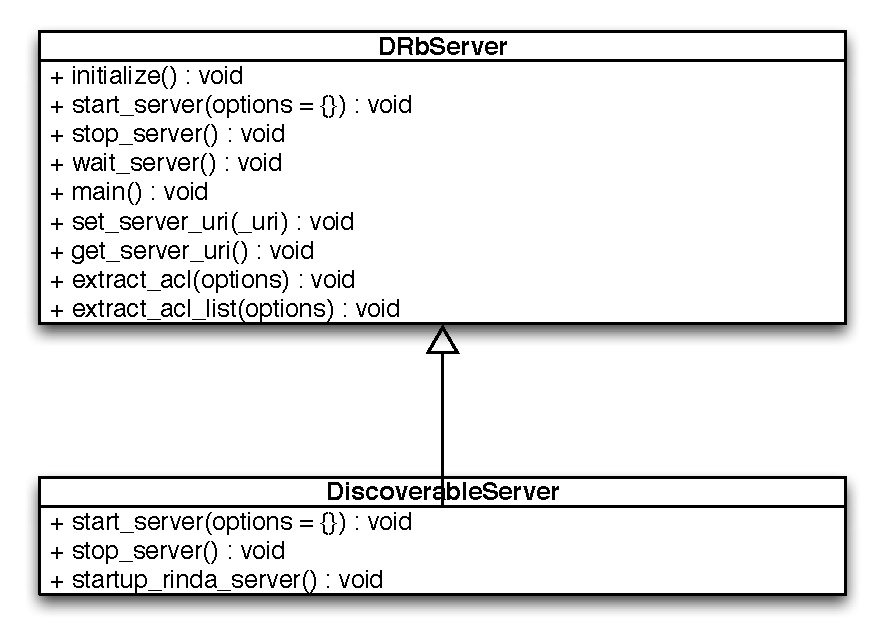
\includegraphics[width=0.6\textwidth]{images/detail/drbserver_class.eps}
\caption{DRbServer及DiscoverableServer类图}
\label{fig-drb-class}
\end{figure}

MessageServer使用DRb技术实现远程过程调用,利用Rinda技术实现服务器的自动发现。DRbServer则是封装了一个用于实现DRb协议的实体类,其接口作用分别如下所示:

initialize是DRbServer类的构造函数,负责构造和初始化DRbServer类。start\_server负责开启DRb服务器,他的调用将使得DRbServer开始监听本地端口,从而相应远方请求。该接口同时接受一个可选参数,该参数是一个哈希表类型,用acl:作为其键,其值表示一个ACL(Access Control List)列表。该列表的提供主要是基于安全方面的考量,该列表制定了一系列规则,指明了哪些远程主机能够访问本地DRb服务哪些将被拒绝。stop\_server接口则是负责停止DRbServer工作,从而使得本机不再相应远程请求。wait\_server则使执行线程被挂起,等待DRb服务器执行完成,直到其停止执行,方才返回。

main接口主要用作调试,它使得DRbServer拥有一个入口函数,从而使得能够简单的引用改代码从而使得DRb服务器能够执行。set\_server\_uri和get\_server\_uri用于设置和获取DRb服务器的URI。值得指出的是,set\_server\_uri需在DRbServer实际运行之前得以执行,这样DRbServer开启之后便会监听指定的端口,而后者则需要在DRbServer运行之后执行,用于获取当前DRbServer监听的端口。最后,extract\_acl和extract\_acl\_list则与ACL有关,主要用于控制和提取参数中的ACL信息。

DiscoverableServer正如其名所暗示的,负责自动发现服务器。这项机制通过Rinda技术得以实现。由于DiscoverableServer继承于DRbServer,因此大部分的行为和接口语义都和后者一致。除了接口startup\_rinda\_server,他是DiscoverableServer才有的,负责开启一个Rinda服务器,从而支持服务器自动发现。

上面两个类为MessageServer提供了基础的实现技术,为了使得这两个接口更加便于使用,本技术还提供了一套统一的接口,该接口可以被DRb服务器、Rinda以及DRb客户端同时使用。其设计类图见图\ref{fig-msg-server-class}

\begin{figure}[h]
\centering
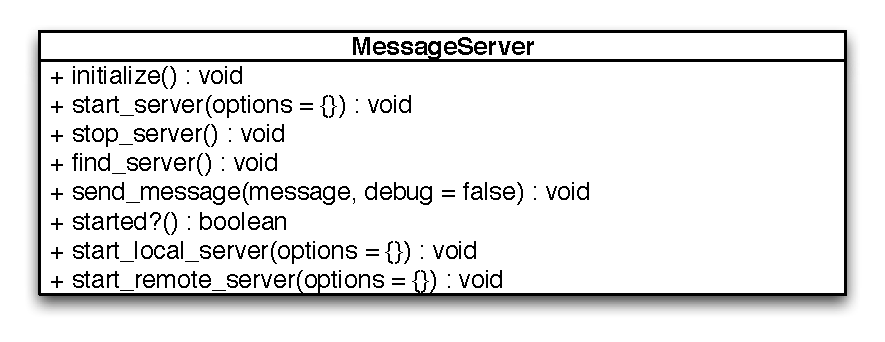
\includegraphics[width=0.6\textwidth]{images/detail/message_bus_class.eps}
\caption{MessageServer类图}
\label{fig-msg-server-class}
\end{figure}

在图\ref{fig-msg-server-class}中,initialize是DRbServer类的构造函数,负责构造和初始化MessageServer类。start\_server负责开启一个DRb服务器和Rinda服务器,该接口接收一个参数,该参数提供了额外的配置信息。该参数是一个哈希表,其中acl的键表明了该服务器的ACL规则,deploy的表明了本服务器的部署方式。就目前而言,MessageServer提供了两种方式,一种是InProc,若使用该种方式,则DRb和Rinda服务器就直接运行在当前进程之中;另一种是StandAlone,若使用这种方式,则DRb和Rinda服务器将运行在一个新建的子进程之中,从而能够很好的和父进程隔离起来,避免一些安全性和稳定性的问题。虽然启动服务器时需要区分InProc和StandAlone两种配置方式,但是在使用接口stop\_server接口停止服务器时则不需要作此区分,该接口会自动针对不同种类服务器作出相应行为,以停止其运行。

一般来说,只能有一个DRb和Rinda服务器。对于客户端,虽然给予API统一性的考虑依然使用MessageServer类,但是这些客户端却不能使用star\_server,因为其只能作为DRb服务器的消费者。因此,为了首先找到可用的DRb服务器,他们需要首先调用find\_server接口,该接口会自动使用Rinda技术找到服务器,这之后才能够向MessageServer发送请求。由于服务器可能随时关闭,因此MessageServer同样提供了一套接口用于查询服务器运行状态。started?接口返回一个布尔值,改值指明了当前是否有DRb服务器,如果有,该服务器是否正在运行,能否服务等问题。

send\_message是最为重要的接口,他是MessageServer的服务接口。MessageServer本来旨在让服务器进程代理非服务器进程的消息传递任务,而这个接口便是非服务器进程请求的通道。该接口接收两个参数,其一是待发送的消息,另外则是一个标记,用于开启或者关闭在控制台写调试信息这一行为。值得指出的是,消息不仅仅只是字串,消息能够使任意Ruby对象,这样能够大大增加程序的灵活性,降低对特定类型的耦合。

最后start\_local\_server和start\_remote\_server两个接口属于辅助接口,其分别对应InProc和StandAlone两种配置的服务器。他们这两个接口一般是不需要用户主动调用的。

\begin{figure}[h]
\centering
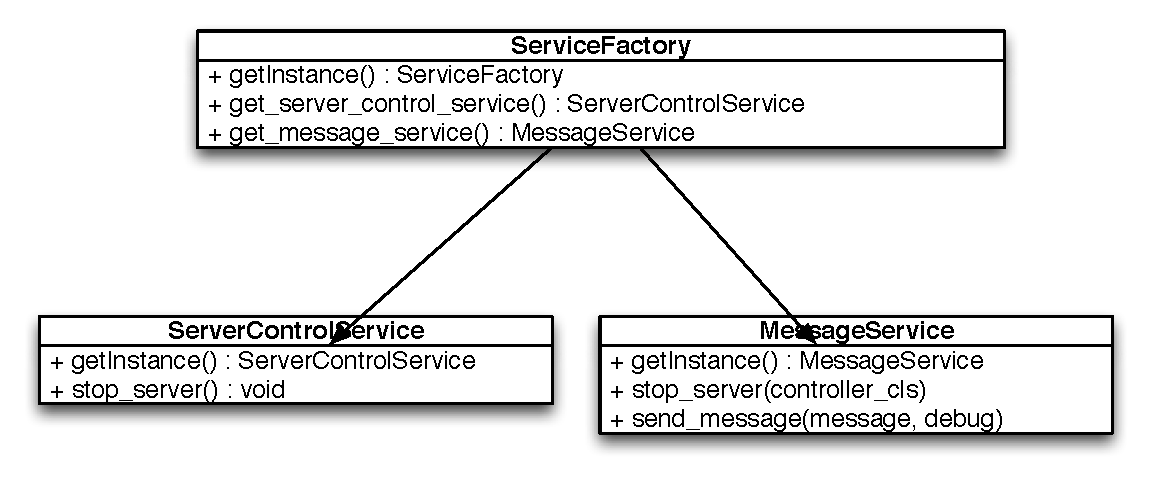
\includegraphics[width=0.7\textwidth]{images/detail/factory_class.eps}
\caption{DRb服务工厂类图}
\label{fig-factory-class}
\end{figure}

图\ref{fig-factory-class}展示了DRb服务器工厂类的结构。根据DRb协议内容,每个DRb服务器需要有一个前置对象(Front Object),于是本系统使用一个类工厂作为该前置对象。客户通过DRb API直接获取工厂对象,再通过工厂对象获取其他对象,从而实现远程执行逻辑。目前,工厂提供了两个类,一个负责远程控制DRb服务器,另一个负责支持远程消息传递服务。

对于ServiceFactory类来说,其使用了单例设计模式。通过getInstance的调用,可以获取这个实例。get\_server\_control\_service接口则是用于获取一个ServerControlService对象,从而控制远程DRb服务器。get\_message\_service接口则是用于获取一个MessageService对象,从而能够通过服务器进程向浏览器发送消息。

对于ServerControlService类来说,亦使用了单例设计模式,因此getInstance同样用于获取一个实例。stop\_server则供远程调用,以终止DRb服务器的运行。MessageService类的getInstance用于获取单例实例。其send\_message接口则用于远程方向本地请求发送消息,本地服务器接收到请求后,便会通知相应前端,向浏览器发送消息。为了知道通过哪个前端控制器向客户端发送数据,相应的控制器需要首先调用egister\_reload\_handler接口,从而将自己注册给本系统,使得本系统能够通知其发送消息。

\subsubsection{工作流程}
图\ref{fig-msg-process}展示了MessageServer的基本工作流程:
\begin{figure}[h]
\centering
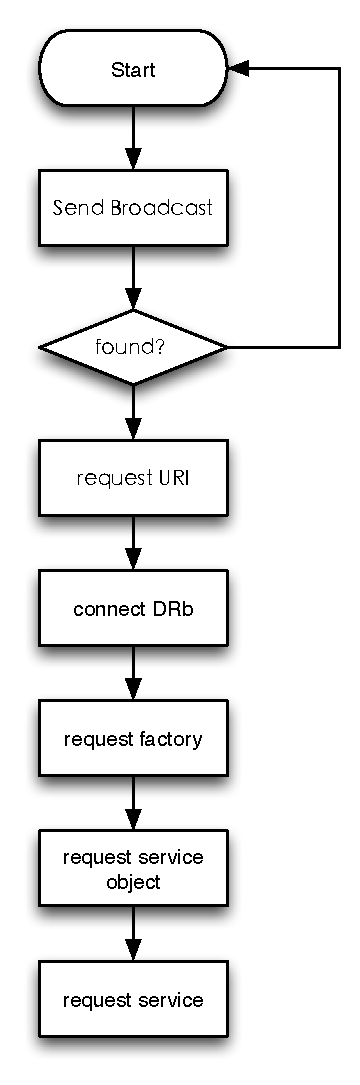
\includegraphics[width=0.3\textwidth]{images/detail/message_server_process.eps}
\caption{MessageServer工作流}
\label{fig-msg-process}
\end{figure}

在系统初始化时,首先需要发送一个广播的数据包,这个广播报文将被Rinda服务器收到,并告知自己的存在。系统接收到Rinda服务器的存在消息之后,便会向Rinda服务器请求本地DRb服务器的URI地址。Rinda服务器接收到该请求之后,便会将之前向自己注册的DRb服务器的地址传送给系统。系统接收到URI数据之后,便会尝试连接该URI,从而和DRb服务器建立了连接。在和DRb服务器建立连接之后,系统将向其请求一个前端对象。此时,系统获得的前端对象实际上是一个工厂,因此系统将向该工厂请求其他的服务对象。目前来说,有两个对象,一个负责控制DRb服务器的运行,另一个负责发送实时消息。系统获得服务对象之后,便通过相应服务对象的接口,实现相应的功能。


\subsubsection{关键代码}
MessageServer的主要逻辑如代码\ref{msg-server-core}所示:
\begin{lstlisting}[caption={MessageServer核心代码展示}, label=msg-server-core]
class MessageServer
  include Singleton

  def start_server(options = {})
    @is_owner_process = true

    method = extract_deploy_method(options)
    if method == :InProc
      @is_in_proc_server = true
      start_local_server(options)
    else #method == :StandAlone
      @is_in_proc_server = false
      start_remote_server(options)
    end
  end

  def stop_server
    raise RuntimeError, 'call find_server first' unless @server_uri

    services = DRbObject.new_with_uri @server_uri
    controller = services.get_server_control_service
    controller.stop_server

    reset_params_when_stop
  end

  def find_server
    if !(@is_owner_process && @is_in_proc_server)
      DRb.start_service 
    end

    finger = Rinda::RingFinger.new nil, DiscoverableServer::DEFAULT_PORT
    ring_server = finger.lookup_ring_any
    @server_uri = ring_server.__drburi
  end

  def send_message(message, debug = false)
    raise RuntimeError, 'call find_server first' unless @server_uri

    services = DRbObject.new_with_uri @server_uri
    
    msg = services.get_message_service
    msg.send_message(message, debug)
  end

  def started?
    server_exist = false
    begin
      @soc = UDPSocket.open
      @soc.bind("", DiscoverableServer::DEFAULT_PORT)
      @soc.close
    rescue Errno::EADDRINUSE
      server_exist = true
    end

    server_exist
  end
end
\end{lstlisting}


\subsection{ActionController::Live设计}
\subsubsection{接口设计}
ActionController::Live是负责Rails消息总线技术中负责底层数据实时传输的类,该类使用Rack劫持技术,使得上层逻辑能够绕开服务器对套接字的管理,从而向套接字任意的发送数据。该类的主要类结构如下图所示:

\begin{figure}[h]
\centering
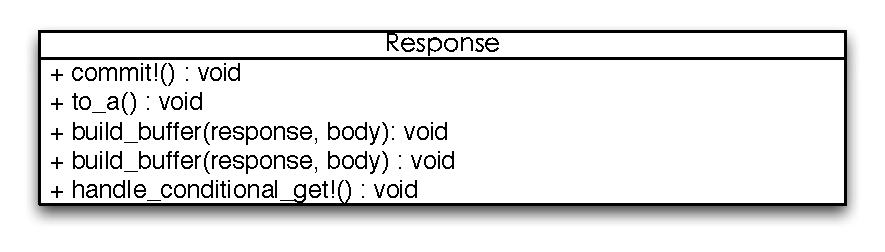
\includegraphics[width=0.7\textwidth]{images/detail/response_class.eps}
\caption{Response对象类图}
\label{fig-response-class}
\end{figure}

Reponse实体类是模拟Rails框架中HTTP相应的实体类,它提供了一系列方法用于表示一个HTTP相应并储存其数据内容。Response类实际上继承自Rails系统的相应对象。commit!方法用于向Rails指出该响应目前已经构建完成,可以提交(发送至)浏览器客户端。t\_a这个接口是将Ruby类表示的HTTP响应对象序列化为字节流,这之后才能通过相应的数据发送模块将响应数据反馈回浏览器。build\_buffer方法用于生成一个Buffer对象,该对象用于缓存数据,从而能够提高网络IO工作效率。merge\_default\_headers这个方法主要用于合并参数中的HTTP头中的数据到自身,从而起到一个覆盖或者说重载数据的作用。handle\_conditional\_get主要是为了在客户端浏览器发送HTTP conditional GET请求的时候能够正确关闭相应对象而设计的接口。

\begin{figure}[h]
\centering
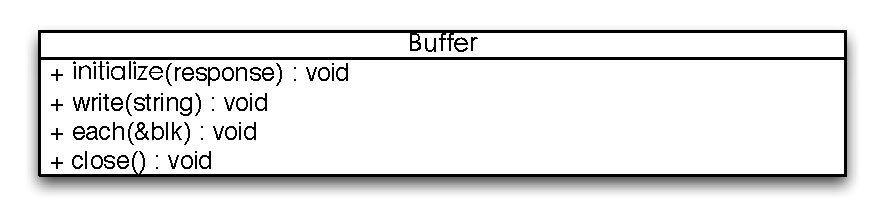
\includegraphics[width=0.7\textwidth]{images/detail/buffer_class.eps}
\caption{Buffer对象类图}
\label{fig-buffer-class}
\end{figure}

Buffer类主要提供了一套缓存机制,从而使得数据能够被缓存至一定时机方才将数据发送,最终提高了网路IO的工作效率。Buffer的initialize接口同样是其构造和初始化时调用的函数,接受一个Response对象实例,用于正确同步和Response的数据。write接口用于该缓存写入数据,该接口接受一个任意对象,将调用对象的to\_s方法从而获取一个string对象,并将其写入到缓冲区里。each接口用于读取缓存内容,Buffer并没有提供直接的字节级别的访问方式,而是使用each提供了给予块的访问方式。该方法接收一个Block对象,该对象将会在每轮迭代时被调用,并被传入缓存中的数据。close方法用于不使用缓存时将缓存关闭,从而回收系统资源防止资源泄露。

\begin{figure}[h]
\centering
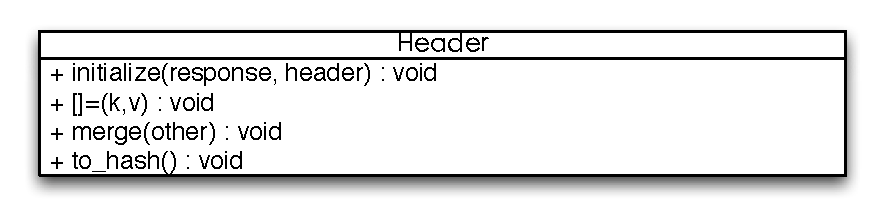
\includegraphics[width=0.7\textwidth]{images/detail/header_class.eps}
\caption{Header对象类图}
\label{fig-header-class}
\end{figure}

Header类主要封装了HTTP数据报文中HTTP报头的数据,使得其可以通过面向对象的方式访问,而不需要手动解析ASCII数据流。该方法提供了的initialize接口接口接收一个response对象,并且初始化相应的状态。[]=方法用于提供对HTTP报头中对应数据域中数据的读写。merge方法则是提供了合并两个HTTP包头数据的工作,其参数是被合并进来的报头数据。to\_hash接口负责将Header对象转化为一个哈希表对象。

\begin{figure}[h]
\centering
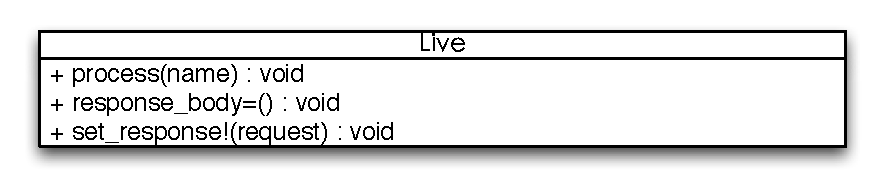
\includegraphics[width=0.7\textwidth]{images/detail/live_class.eps}
\caption{Header对象类图}
\label{fig-live-class}
\end{figure}

Live模块主要负责改变Rails Controller对象原有的行为方式。这里的三个方法都是重载方法,他们改变了Rails原生控制器,使得其开始支持实时数据。process接口是负责响应浏览器HTTP请求是被调用,并产生HTTP响应的函数。response\_body=方法则主要是负责设置当前控制器的HTTP响应对象。set\_response对象则是负责设置控制器所关联的HTTP响应对象的状态到标准值。

\subsubsection{工作流程}
Live模块的主要工作流程如图\ref{fig-live-process}所示:

\begin{figure}[h]
\centering
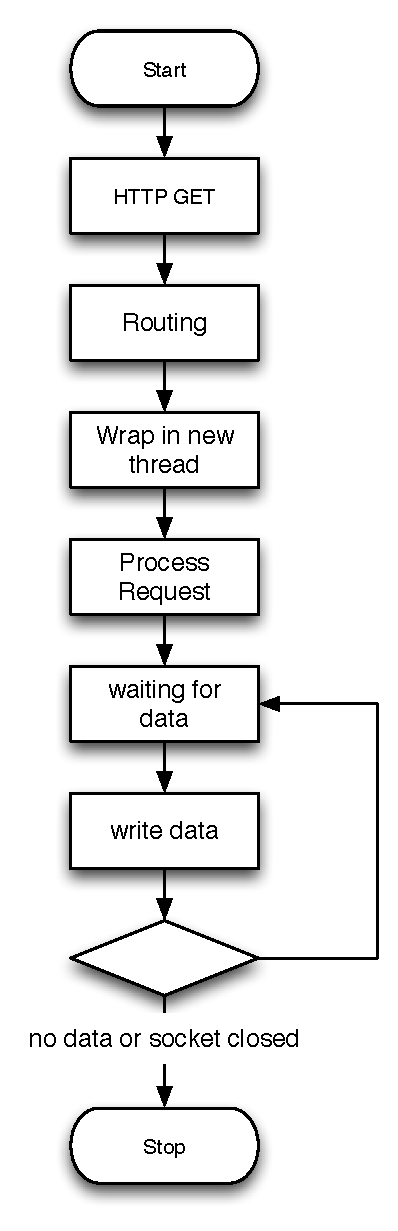
\includegraphics[width=0.27\textwidth]{images/detail/live-process.eps}
\caption{Live模块工作流程}
\label{fig-live-process}
\end{figure}

不难看到,到Rails接收到HTTP GET请求之后,便会根据相应路由规则将该请求路由给相应的控制器实例。控制器接收到请求之后,首先会将处理过程委托给一个新线程,然后立刻返回处理请求。这之后,控制器等待子线程的数据,一旦接收到任何数据则将立刻发送给客户端。这个过程将一直重复,直到客户端切断连接导致套接字关闭,或者上层逻辑显式地关闭数据流。



\subsubsection{关键代码}
Live的主要逻辑如代码\ref{live-core}所示:
\begin{lstlisting}[caption={Live核心代码展示}, label=live-core]
def process(name)
  t1 = Thread.current
  locals = t1.keys.map { |key| [key, t1[key]] }

  # This processes the action in a child thread. It lets us return the
  # response code and headers back up the rack stack, and still process
  # the body in parallel with sending data to the client
  Thread.new {
    t2 = Thread.current
    t2.abort_on_exception = true

    # Since we're processing the view in a different thread, copy the
    # thread locals from the main thread to the child thread. :'(
    locals.each { |k,v| t2[k] = v }

    begin
      super(name)
    ensure
      @_response.commit!
    end
  }


  raise NotImplementedError, "ActionController::Live requires rack hijack support" unless @_env["rack.hijack?"]
  response.headers["rack.hijack"] = lambda do |io|
    Thread.new {
      begin
        response.stream.each do |part|
          io.write part
        end
      ensure
        response.stream.close
        io.close
      end
    }
  end

  @_response.await_commit
end
\end{lstlisting}

\subsection{ActionControler::ServerSentEvents设计}
\subsubsection{接口设计}
ActionControler::ServerSentEvents负责提供SSE消息语义及其实现,目前提供了两种级别的SSE实现。该模块包含的类结构如下所示:

\begin{figure}[h]
\centering
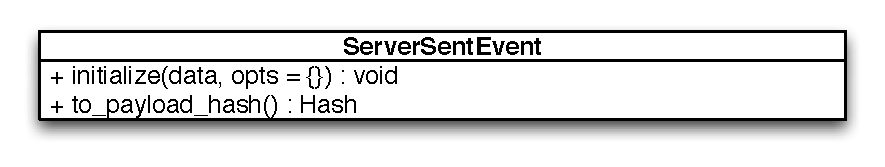
\includegraphics[width=0.7\textwidth]{images/detail/sse_class.eps}
\caption{ServerSentEvent对象类图}
\label{fig-sse-class}
\end{figure}

ServerSentEvent对象主要用于封装一个SSE消息体,该对象主要有两个接口,其中initialize接口负责初始化这个对象。该接口接收两个参数,第一个参数是消息数据本身,第二个参数是SSE消息选项。根据SSE标准协议,这些选项可能是name,id以及retry等,这些参数将通过哈希表的形式组织起来,并且通过第二个参数传入。

\begin{figure}[h]
\centering
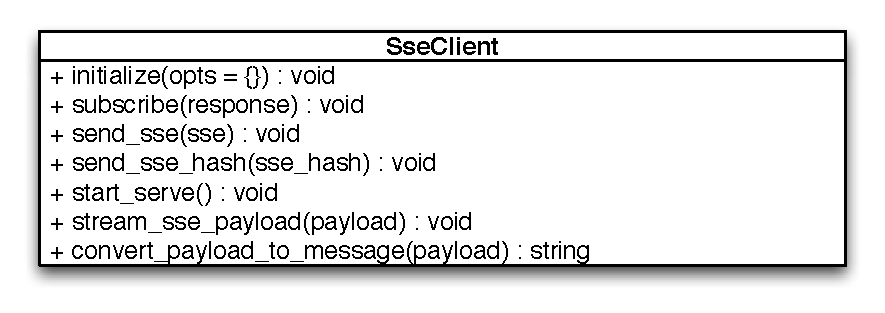
\includegraphics[width=0.7\textwidth]{images/detail/sse_client_class.eps}
\caption{SseClient对象类图}
\label{fig-sseclient-class}
\end{figure}

SseClient对象主要负责同特定客户端实现SSE详细推送,该对象主要接口如下:首先,initialize接口负责初始化这个对象,该接口接受一个哈希表为参数,该参数主要用于参与设置该类的初始化状态设置,其中subscribe域设置该对象中包含的HTTP数据流对象,start\_on\_initialize域则表示一旦初始化这个对象则立刻开始尝试和浏览器客户端建立连接。send\_sse接口用于向客户端浏览器发送一个SSE消息体,该接口接受一个参数,这个参数是ServerSentEvent实例对象,包含了欲发送的数据内容。另一个接口是send\_sse\_hash接口,该接口和send\_sse接口类似,用于发送消息其唯一的不同在于,该接口接收一个哈希表,其中data键下的数据即为待传输的数据实体。start\_serve的调用会使得主调线程陷入阻塞态,此时线程等待其他线程写入数据,一旦检测到数据写入,该线程则立刻将数据传送给客户端浏览器,实现数据的实时传送。stream\_sse\_payload该方法接受一个ServerSentEvent对象,并将其传送给浏览器客户端。convert\_payload\_to\_message接口则负责将一个ServerSentEvent对象系列化,转换为字节流并返回。

\begin{figure}[h]
\centering
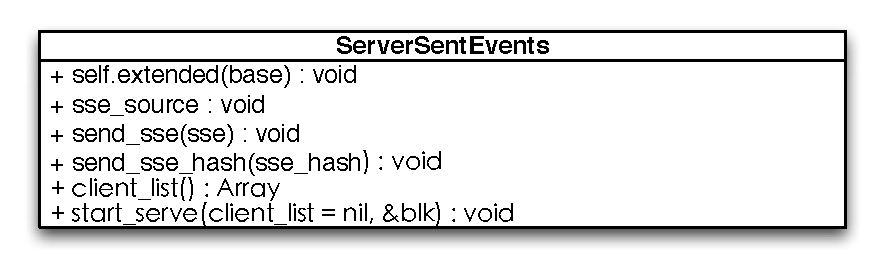
\includegraphics[width=0.7\textwidth]{images/detail/sses_class.eps}
\caption{ServerSentEvents对象类图}
\label{fig-sses-class}
\end{figure}

ServerSentEvents主要负责重载控制器原有行为方式,从而提供适合于实时数据传送的行为。其中,self.extended接口是一个回调函数,任何使用该模块的控制器都会调用它,该接口将把主调类注册至其内部变量,供控制器级别的SSE使用。sse\_source接口是一个自动定义接口,任何使用ServerSentEvents模块的控制器类都会获得这个函数的定义,用于处理控制器级别的SSE消息。send\_sse和send\_sse\_hash则主要是向所有访问该控制器的浏览器客户端发送SSE消息。client\_list则是当前所有连接到本控制器的浏览器客户端列表。start\_serve接口主要负责监听端口和传输数据。

\subsubsection{工作流程}
ServerSentEvents模块的主要工作流程如图\ref{fig-sses-process}所示:

\begin{figure}[h]
\centering
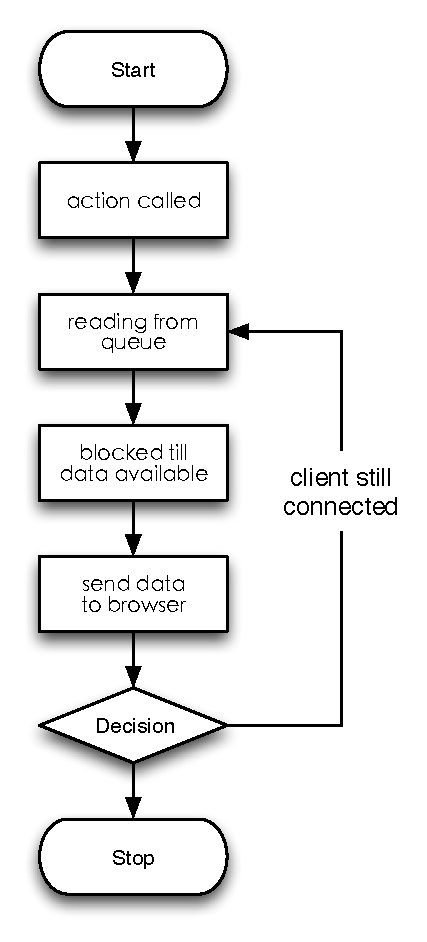
\includegraphics[width=0.27\textwidth]{images/detail/sse_process.eps}
\caption{ServerSentEvents模块工作流程}
\label{fig-sses-process}
\end{figure}

首先,当浏览器向特定控制器请求接收SSE消息时,该控制器相应的action处理例程被调用了,接下来该例程会进行一系列初始化过程,这之后便会从一个数据队列中循环读取消息,如果没有消息则线程陷入阻塞状态直到有数据到达数据队列。一旦获取数据,该模块便会将数据构造为SSE对象,并序列化为合适的字节流表示方式同时构造HTTP响应数据流,并通过Live模块的实时传输功能将数据传输给浏览器客户端。而一旦发觉浏览器关闭了和服务器的链接,本模块则即刻退出,否则继续等待数据。

\subsubsection{关键代码}
ServerSentEvents的主要逻辑如代码\ref{sses-core}所示:
\begin{lstlisting}[caption={ServerSentEvents核心代码展示}, label=sses-core]
module ServerSentEvents
  OPTIONAL_SSE_FIELDS = [:name, :id, :retry]
  REQUIRED_SSE_FIELDS = [:data]

  SSE_FIELDS = OPTIONAL_SSE_FIELDS + REQUIRED_SSE_FIELDS

  module ClassMethods
    @@sse_clients = {}

    def self.extended(base)
      base.class_exec do
        # the entry point for a Controller level SSE source
        def sse_source
          start_serve self.class.client_list
        end
      end
      @@sse_clients[base] = []
    end

    def send_sse(sse)
      client_list.each do |client|
        begin
          client.send_sse(sse)
        rescue IOError
        end
      end
    end

    def send_sse_hash(sse_hash)
      client_list.each do |client|
        begin
          client.send_sse_hash(sse_hash)
        rescue IOError
        end
      end
    end

    def client_list
      @@sse_clients[self]
    end
  end

  def start_serve(client_list = nil, &blk)
    client = SseClient.new
    client.subscribe response
    client_list << client if client_list

    Thread.new do 
      begin
        blk.call client if block_given?
      ensure
      end
    end

    client.start_serve
  ensure
    client_list.delete_if {|it| it == client} if client_list
    response.stream.close
  end
end
\end{lstlisting}

\section{Auto Reload和Backend Instrumentation的设计}
\subsection{FileSystemChecker设计}
\subsubsection{接口设计}
FileSystemChecker类是负责监控特定目录,并且通知特定模块该目录文件系统发生变动的类。该类的定义如图\ref{fig-fuc-class}

\begin{figure}[h]
\centering
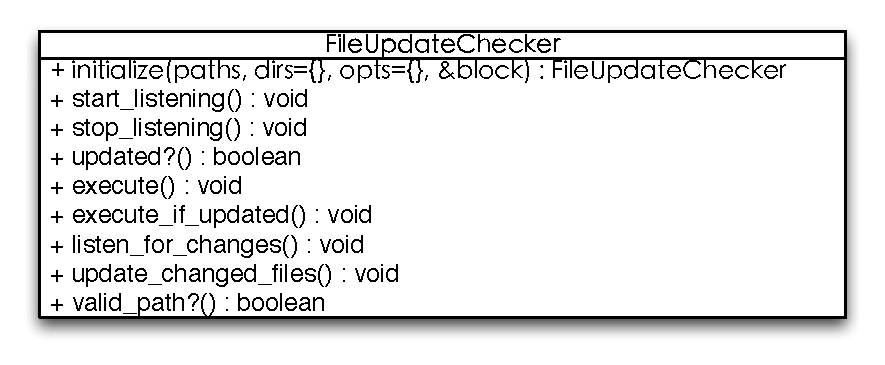
\includegraphics[width=0.6\textwidth]{images/overview/file_update_checker_class.eps}
\caption{FileSystemChecker类图}
\label{fig-fuc-class}
\end{figure}

图\ref{fig-fuc-class}描述了该类所具有的接口,其中initialize接口是该类的构造函数,负责初始化该类的状态。这个接口可接受三个参数,第一个参数是一个数组,该数组包含了所有待监视的目录名。第二个参数是可选参数,它包括了一个哈希表,哈希表是以前一个参数中包含的各个目录名为键,对应的值是一个包含文件拓展名的数组,借此告知FileSystemChecker在对应目录下仅监视该拓展名的文件变动事件。第三个参数则是传入初始化选项,是一个哈希表,它支持如下这些选项:

\begin{itemize}
\item :filter。指明一个正则表达式,使得FileSystemChecker仅仅监视文件名符合该表达式的文件
\item :ignore。指明一个正则表达式,使得FileSystemChecker忽略文件名和该表达式匹配的文件。
\item :notification。指明一个包含Notification名字的数组,当文件变动时FileSystemChecker负责引发这些Notification,这时候如果这个Notification有相应的观察者,则这些观察者将最终收到FileSystemChecker的文件系统变动通知。
\item :recurse。如果该参数为真,则FileSystemChecker会同时监控指明目录的所有子目录。通过对该目录进行深度优先搜索,所有该文件树的文件文件夹新建、修改、删除等事件都能被监控。
\end{itemize}

最后,initialize接口还接受一个Block,这个Block会在每次文件变动被检测到或者execute和execute\_if\_updated被调用是被执行。

start\_listening函数指示FileSystemChecker开进监控文件系统的变动。一旦调用这个方法,程序将会陷入阻塞态,直到其他线程中的代码调用stop\_listening。相应的,stop\_listening负责停止FileSystemChecker对某个文件夹的监控。值得指出的是,一旦FileSystemChecker停止监控后在下一次开始监控时,会将期间所有文件变动通知给消息订阅者。

updated?返回一个布尔值,知名当前是否有文件发生变动,execute将会引发传给构造函数的block的执行,并且会再次检查文件系统是否变动,execute\_if\_updated则是仅仅在有文件变动的前提下执行block。

listen\_for\_changes是监控文件系统的实现函数,这个函数使用深度优先搜索方式搜索文件系统,并且找到文件系统的变动。update\_changed\_files负责实现深度优先搜索。

\subsubsection{工作流程}
图\ref{fig-fuc-process}展示了FileSystemChecker工作的主要流程:

\begin{figure}[h]
\centering
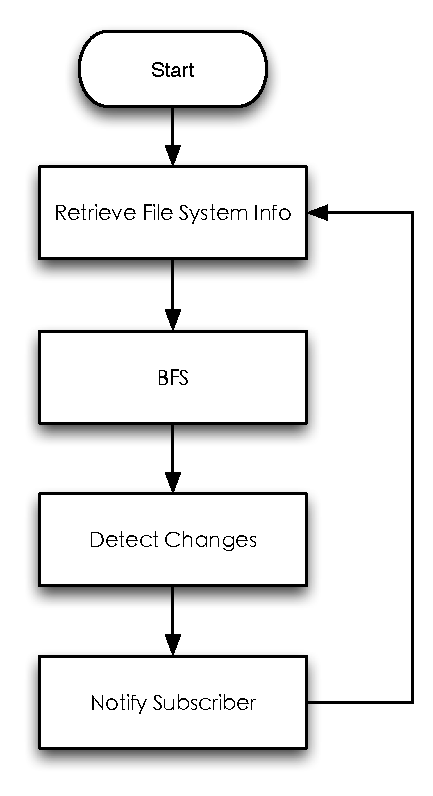
\includegraphics[width=0.3\textwidth]{images/detail/fuc_process.eps}
\caption{FileSystemChecker工作流程图}
\label{fig-fuc-process}
\end{figure}

可以看到,FileSystemChecker在开始监控目录后是以无限循环的形式工作的,在每次循环之前,都会首先获取被监视文件系统的文件信息。实际上,该步骤是给文件系统拍摄快照,用于捕获其当前状态。这之后,FileSystemChecker会对合格树形结构的数据集合进行一个深度优先搜索,通过此实现对所有文件节点的比对。在这之后,FileSystemChecker将当前快照数据同该模块上一次捕获的快照进行比较,借此找出其不同。这些不同则是上次快照捕获到此时文件系统的变化,于是FileSystemChecker便能够即刻发现操作系统文件的变化。当发觉一个或者多个变化后,FileSystemChecker接下来便会通过Notification通知观察者该项变动。值得指出的是,Notification机制是Rails框架内早已存在的一项服务器内部通用消息传送方案,观察者需要首先向某个Notification注册自己,让后方能接收到FileSystemChecker发送的文件变动消息。

\subsubsection{关键代码}
代码\ref{fuc_core}展示了FileSystemChecker的核心实现:
\begin{lstlisting}[caption={FileSystemChecker核心代码展示}, label=fuc_core]
# Starts listening to changes in the filesystem. This method is
# synchronized until the stop_listening method is called. Once the object
# starts listening, it goes through and checks all files that have been
# changed since the object was created.
#
# If the object was previously stopped, and start_listening is called
# again, then all of the file changes since the last stop was called will
# be pushed to the changed_files queue. The files which were created and
# deleted between the stop and start of the method will be ignored.
def start_listening
  @continue_listening = true
  while @continue_listening
    listen_for_changes
    sleep(0.5)
  end
end

def listen_for_changes
  @semaphore.synchronize do
    @files_alive = []

    paths = initialize_paths(@paths, @dirs)
    directories = handle_paths(paths)
    if @opts[:recurse]
      update_changed_files(directories)
    end

    deleted_files = @file_cache.keys - @files_alive.uniq
    deleted_files.each do |filename|
      @file_cache.delete(filename)
      push_changes(filename, :removed)
    end
  end
end

def update_changed_files(directories)
  new_directory_paths = []

  directories.each do |directory_path|
    expanded_filepaths = Dir.foreach(directory_path)
    .reject { |path| path == ".." || path == "." }  # reject up and self directories on UNIX
    .map { |path| "#{directory_path}/#{path}" }

    new_directory_paths += handle_paths(expanded_filepaths)
  end

  update_changed_files(new_directory_paths) if new_directory_paths.any?
end
\end{lstlisting}

\subsection{MessageBus及Instrument Gem设计}
\subsubsection{接口设计}
MessageBus Gem是Rails消息总线技术中负责初始化Auto Reload模块的功能,并提供以Railtie的形式的初始化插件。Instrument Gem则是本系统中负责提供后台性能数据评估和收集的模块,该模块同时提供了相应的初始化功能,并且同样以Railtie的形式将其插件化。这两个类的主要类结构如下图所示:

\begin{figure}[h]
\centering
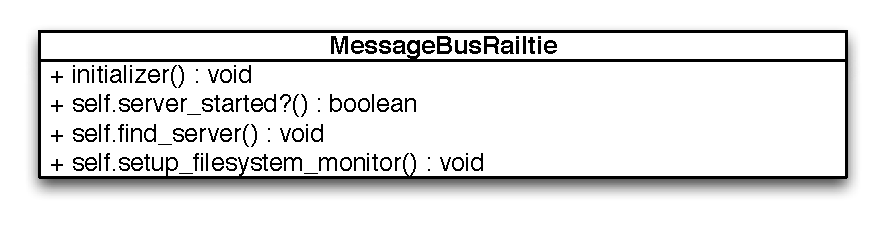
\includegraphics[width=0.7\textwidth]{images/detail/autoload_class.eps}
\caption{MessageBus Gem对象类图}
\label{fig-autoload-class}
\end{figure}

可以看到,MessageBus Gem主要是由四个接口构成的。首先是initializer接口,该结构并非其构造函数或是类初始化接口,而是作为Railtie整体框架下的一个回调函数。因为MessageBus Gem使用了Railtie技术,作为Railtie初始化进程,在整个Rails初始化时会依次调用所有Railtie的的初始化回调方法,则此时MessageBus Gem相应方法将被调用,从而实现该模块的初始化。self.server\_started?接口返回一个布尔值,该值指出目前DRb服务器是否开启。self.find\_server则是负责调用底层代码,实现自动发现本地的DRb服务器的逻辑。self.setup\_filesystem\_monitor则是负责开启FileUpdateChecker模块,使之开始监控Rails工程目录,并注册相应回调函数。

\begin{figure}[h]
\centering
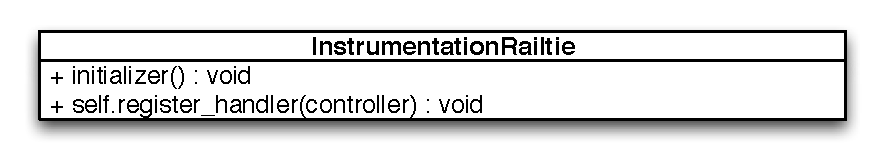
\includegraphics[width=0.7\textwidth]{images/detail/instrument_class.eps}
\caption{Instrument Gem对象类图}
\label{fig-instrument-class}
\end{figure}

可以看到,Instrument Gem主要是由两个接口构成的。首先是initializer接口,该结构并非其构造函数或是类初始化接口,而是作为Railtie整体框架下的一个回调函数。因为Instrument Gem同样使用了Railtie技术,作为Railtie初始化进程,在整个Rails初始化时会依次调用所有Railtie的的初始化回调方法,则此时Instrument Gem相应方法将被调用,从而实现该模块的初始化。self.register\_handler则是负责注册一个控制器,该控制器会在本模块收集到性能数据后作为目标将数据发送之。

\subsubsection{工作流程}
本模块的主要工作流程如图\ref{fig-gem-process}所示:

\begin{figure}[h]
\centering
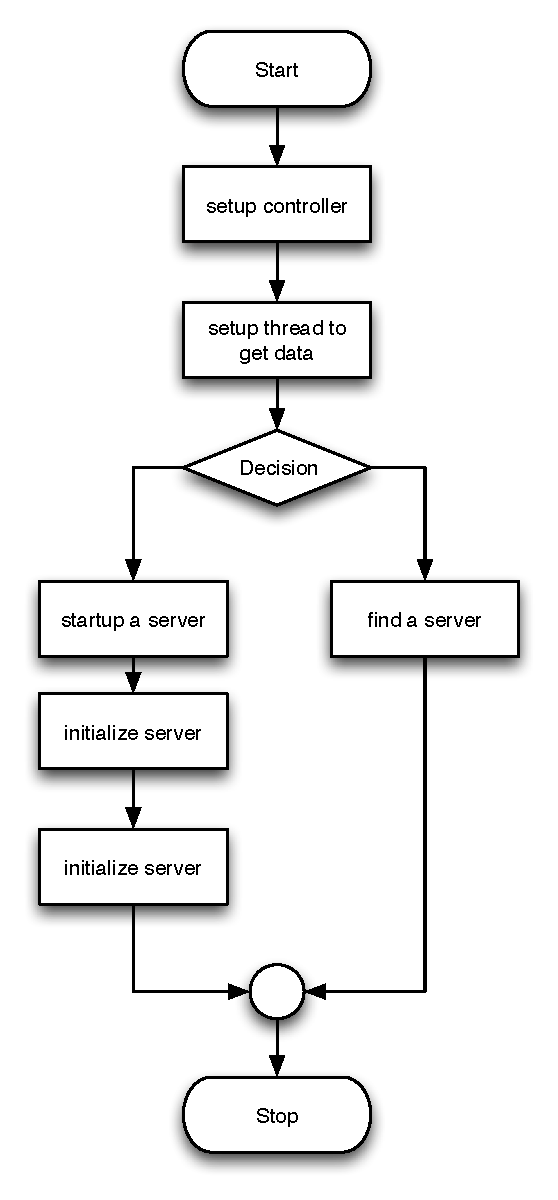
\includegraphics[width=0.35\textwidth]{images/detail/gem_process.eps}
\caption{工作流程}
\label{fig-gem-process}
\end{figure}

在初始化开始的时候,本模块首先会建立相应的控制器,并将其初始化到正确状态。接着,将会新建一个线程,并将任务委托给子线程进行。接下来将会判断当前执行环境,如若是Rails控制台的话,将会自动寻找现已存在的消息总线服务器,接着初始化过程结束;但如果是Rails服务器环境,则会首先建立一个新的消息服务器,接着初始化该服务器和其他相关组件。

\subsubsection{关键代码}
本模块的主要逻辑如代码\ref{gem-core}所示:
\begin{lstlisting}[caption={初始化核心代码展示}, label=gem-core]
require 'rails'

module MessageBus
  class MessageBusRailtie < Rails::Railtie
    private_class_method :new # MessageBusRailtie is not intend to be instantiated

    initializer "message bus initializer" do
      if defined?(Rails::Console)
        flag = MessageBusRailtie::server_started?
        MessageBusRailtie::find_server if flag
      else
        MessageBusRailtie::start_server
        MessageBusRailtie::setup_filesystem_monitor
      end
    end


    def self.server_started?
      server = ActiveSupport::MessageBus::MessageServer.instance
      server.started?
    end

    def self.find_server
      remote_server = ActiveSupport::MessageBus::MessageServer.instance
      remote_server.find_server # broadcast to find local server
    end

    def self.start_server
      server = ActiveSupport::MessageBus::MessageServer.instance
      server.start_server :deploy => :InProc # started in work thread
    end

    def self.setup_filesystem_monitor
      opts = {:notifications => "filesystem_changes", :recurse => true}
      monitor_path = Rails.root

      listener = ActiveSupport::FileUpdateChecker.new([monitor_path], {}, opts)
      Thread.new do
        listener.start_listening
      end

      ActiveSupport::Notifications.subscribe("filesystem_changes") do |*args|
        server = ActiveSupport::MessageBus::MessageServer.instance
        begin
          server.send_message args, true
        rescue Error => err
          puts "Failed to send message.(#{err})"
        end
      end
    end
  end
end
\end{lstlisting}








